\documentclass{article}
\usepackage[paperwidth=330pt,paperheight=250pt,textwidth=250pt,textheight=160pt,top=30pt,left=40pt]{geometry}
\usepackage{dirtreex}
\pagestyle{empty}
\makeatletter
\def\State{\edef\StateNow{\the\parfillskip/\the\parskip/\the\parindent/\the\leftskip/\the\rightskip/\the\baselineskip/\f@size/\f@family/\f@series/\f@shape}}
\def\CheckNode#1{\expandafter\let\expandafter\NodeNow\csname pgf@sh@pi@C\endcsname
\ifx\NodeOld\NodeNow\typeout{ARCH-NODE-#1=PRESERVED}\else\PackageError{namespace-test}{User node #1 was overwritten}{The remembered user node must survive tree output.}\fi}
\def\CheckState#1{\State\ifx\StateBefore\StateNow\typeout{ARCH-STATE-#1=PRESERVED}\else\PackageError{namespace-test}{Outer state #1 changed}{Tree output must restore surrounding state.}\fi}
\begin{document}
\parfillskip=11pt plus 2fil minus 1pt\relax
\parskip=3pt plus 1pt\relax
\parindent=8pt\relax
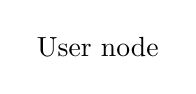
\begin{tikzpicture}[remember picture]\node (C) {User node};\end{tikzpicture}\par
\expandafter\let\expandafter\NodeOld\csname pgf@sh@pi@C\endcsname
\State\let\StateBefore\StateNow
\begin{dirtreex}[pagebreak=false,fontsize={\small\itshape\parfillskip=13pt plus 2fil minus 1pt}]
\dir{ROOT}{ROOT-COMMENT}{\file{N000}{C000}}
\end{dirtreex}
\CheckNode{WHOLE}\CheckState{WHOLE}
\clearpage
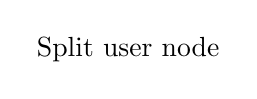
\begin{tikzpicture}[remember picture]\node (C) {Split user node};\end{tikzpicture}\par
\expandafter\let\expandafter\NodeOld\csname pgf@sh@pi@C\endcsname
\begin{dirtreex}[box=false,fontsize={\small\itshape\parfillskip=13pt plus 2fil minus 1pt}]
\dir{SPLITROOT}{SPLIT-COMMENT}{
\file{N001}{C001}
\file{N002}{C002}
\file{N003}{C003}
\file{N004}{C004}
\file{N005}{C005}
\file{N006}{C006}
\file{N007}{C007}
\file{N008}{C008}
\file{N009}{C009}
\file{N010}{C010}
\file{N011}{C011}
\file{N012}{C012}
\file{N013}{C013}
\file{N014}{C014}
\file{N015}{C015}
\file{N016}{C016}
\file{N017}{C017}
\file{N018}{C018}
\file{N019}{C019}
\file{N020}{C020}
\file{N021}{C021}
\file{N022}{C022}
\file{N023}{C023}
\file{N024}{C024}
}
\end{dirtreex}
\CheckNode{SPLIT}\CheckState{SPLIT}
\end{document}
